\subsubsection{Pretraind Models}
\label{experiments:03.1.2:backbone_hippo:pretrained}
\begin{figure}[h!]
    \centering
        \begin{minipage}{0.49\textwidth}
        \centering
        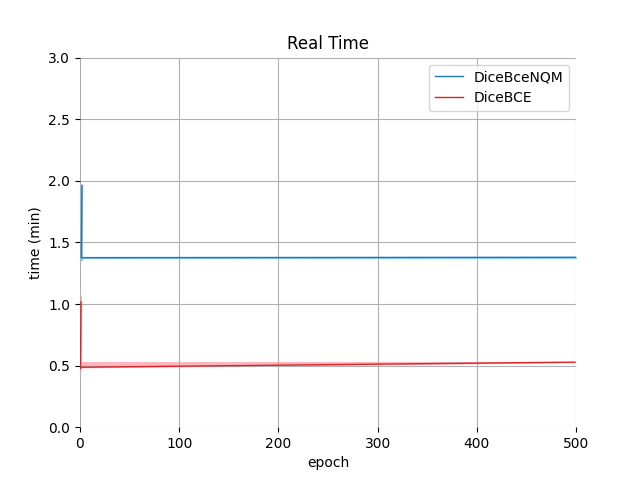
\includegraphics[width=\linewidth]{Graphics/Experiments/3.1.2_realTime_with_error_.png}
    \end{minipage} \hfill
    \begin{minipage}{0.49\textwidth}
        \centering
        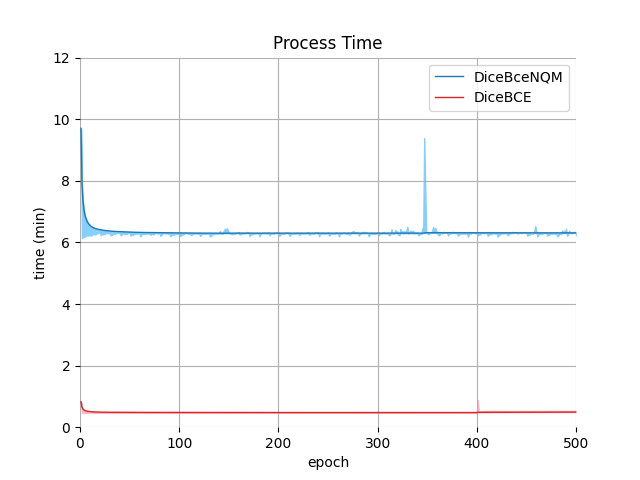
\includegraphics[width=\linewidth]{Graphics/Experiments/3.1.2_process_time_with_errors_.png}
    \end{minipage}
        \caption{Speed comparison between DiceBce and DiceBceNQM for real-time and process time. The average training times per epoch are shown in dark colors. The difference to the actual training times is shown in light colors behind the average. The DiceBceNQM takes much longer to train. The overall means for the real-time are 1.38 min and 0.49 min. The mean values for the process time are 6.33 min and 0.48 min.}
    \label{fig:DiceBCE+NQM:Pretrained:Speedcompare}
\end{figure}

Training on the DiceBceNQM with a stack size of 3 takes about 13.19 times as long as training on the DiceBCE alone and about 2.8 times as long in real time on the system we used (\autoref{experiments:intro:system}, as can be seen in \autoref{fig:DiceBCE+NQM:Pretrained:Speedcompare}). This is simply because with the stacksize, the number of predictions that need to be generated for the NQM is many times greater than without it. We mostly used a stacksize of 3 in our experiments. Therefore, we tested whether we could perform similarly by using pretrained models. To do this, we first trained a cohort of models on the Spike Hippocampus and not augmented datasets. Half of the cohort was trained for the entire 600 epochs on DiceBceNQM. The other half was pretrained for 500 epochs on DiceBCE and another 100 epochs on DiceBceNQM. The results are given in \autoref{tab:3.1.2:DiceBCE+NQM:Pretrained}. The pretrained models are continuously approximately as good as those fully trained on the DiceBceNQM. This is true for the models trained on augmented datasets and those trained on not augmented datasets. The one trained on the non-augmented dataset tends to get a little worse, but compared to the one trained on only 500 epochs \autoref{tab:03.1.1:DiceBCE+NQM_vs_DiceBCE_on_Spike}, both are better on the spike datasets and similar as good on the non-augmented one. Especially for those trained on the sparsely augmented dataset (Spike 0.01), the pretrained performs better rather than worse. 

The equivalence of these training methods is further emphasized when we look at the accumulations of the differences between pretrained and fully trained models for the entire cohort we trained for Dice: The maximum delta was $+ 0.037$, the sum of deltas was $-0.002$, the mean of the absolute deltas was $0.007$, the mean of signed deltas between these two groups was smaller in amount than $0.001$, up to these levels of accuracy. Each for the differences between the two models from the different groups trained on the same datasets (as shown as $\pm$ in the table).
\begin{table}[H]
    \centering
    \begin{tabular}{cl!{\vrule width 1.3pt}llllll}
        \toprule
        \multicolumn{2}{c!{\vrule width 1.3pt}}{model} &
        \multicolumn{5}{c}{\textbf{test dataset} (Dice $\uparrow$)}\\\midrule
        {\bfseries pretrained} & \textbf{train set} & original & Spike 1.0 & Spike 0.3 & Spike 0.2 & Spike 0.1 & Spike 0.01\\\midrule[1.3pt]
        % ---
        no  & original           & 0.881 & 0.662 & 0.812 & 0.811 & 0.858 & 0.881                            \\
        yes & original           & 0.879 & 0.639 -.02 & 0.802 -.01 & 0.801 -.01 & 0.857 & 0.879             \\\rowcolor{BG}
        no  & Spike 1.0          & 0.867 & 0.817 & 0.864 & 0.863 & 0.865 & 0.866                            \\\rowcolor{BG}
        yes & Spike 1.0          & 0.874 +.01 & 0.812 & 0.871 +.01 & 0.867 & 0.872 +.01 & 0.874 +.01        \\
        no  & Spike 0.3          & 0.874 & 0.750 & 0.853 & 0.859 & 0.870 & 0.875                            \\
        yes & Spike 0.3          & 0.872 & 0.757 +.01 & 0.858 +.01 & 0.859 & 0.868 & 0.872                  \\\rowcolor{BG}
        no  & Spike 0.2          & 0.878 & 0.751 & 0.843 & 0.863 & 0.869 & 0.878                            \\\rowcolor{BG}
        yes & Spike 0.2          & 0.879 & 0.727 -.02 & 0.830 -.01 & 0.862 & 0.869 & 0.879                  \\
        no  & Spike 0.1          & 0.875 & 0.754 & 0.849 & 0.860 & 0.869 & 0.876                            \\
        yes & Spike 0.1          & 0.875 & 0.735 -.02 & 0.842 -.01 & 0.855 -.01 & 0.866 & 0.875             \\\rowcolor{BG}
        no  & Spike 0.01         & 0.877 & 0.644 & 0.801 & 0.811 & 0.852 & 0.877                            \\\rowcolor{BG}
        yes & Spike 0.01         & 0.878 & 0.681 \textbf{+.04} & 0.816 +.01 & 0.833 +.02 & 0.861 +.01 & 0.877        \\\bottomrule
    \end{tabular}
    \caption{\textbf{Pretrained Models} (\autoref{experiments:03.1.2:backbone_hippo:pretrained}): Comparrison between pretrained models and full trained ones. For the pretrained models, we used the DiceBCE for the first 500 epochs, since it is faster, and trained after that on the DiceBceNQM for additional 100 epochs. For the not pretrained models we trained full 600 epochs on DiceBceNQM as baseline for the pretrained.\\
    The pretrained models are as good, as the full trained ones. Therefor they can be used to speed up training.}
    \label{tab:3.1.2:DiceBCE+NQM:Pretrained}  
\end{table}